\FloatBarrier

\begin{ilustracion}[ht]
    \centering
    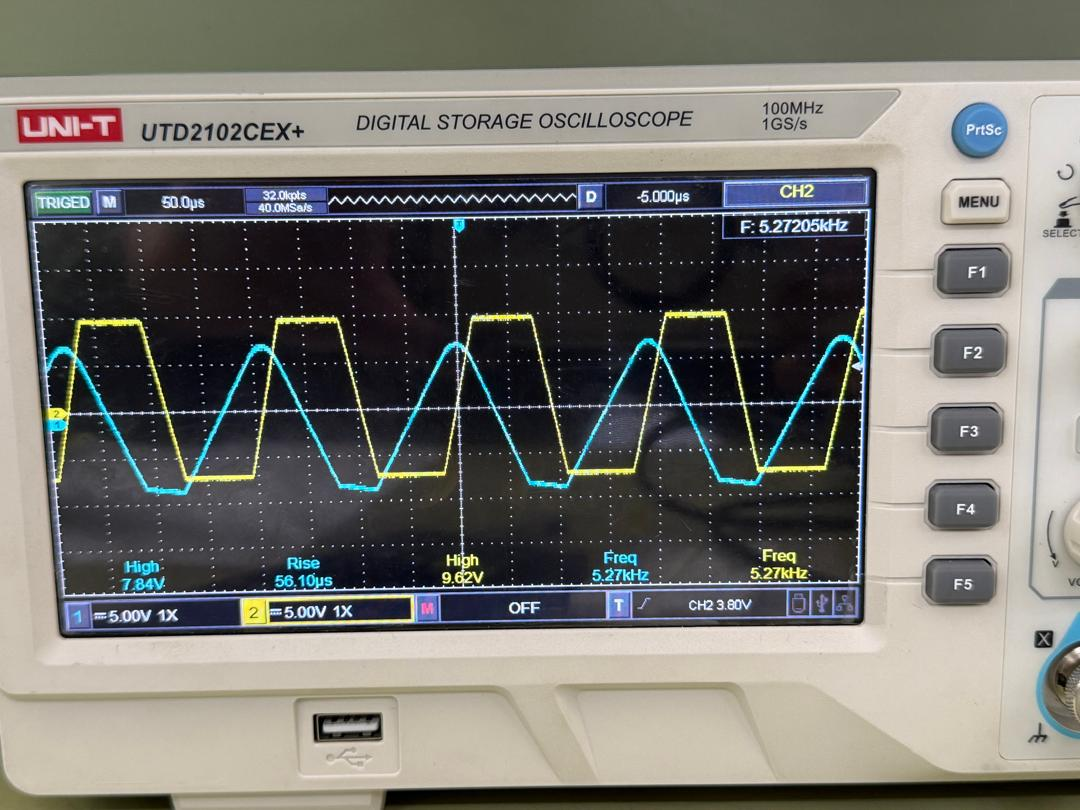
\includegraphics[width=0.6\textwidth]{resultados/generador-funciones.jpg}
    \caption{Medición de voltajes del generador de funciones.}
    \label{ilus:generador-funciones}
\end{ilustracion}

\begin{table}[ht]
\centering
\begin{tabular}{|c|c|c|c|c|c|c|c|c|}
\hline
Descripción & $V_C$ (V) & $\Delta V_C$ (V) & $V_P$ (V) & $\Delta V_P$ (V) & $V_T$ (V) & $\Delta V_T$ (V) & $T$ (s) & $\Delta T$ (s) \\ \hline
Generador funciones & 10.00 & 1.00 & 6.40 & 0.40 & 7.60 & 0.40 & 192.00 & 4.00 \\ \hline
\end{tabular}
\caption{Resultados obtenidos del generador de funciones}
\label{tab:resultados}
\end{table}

\begin{ilustracion}
    \centering
    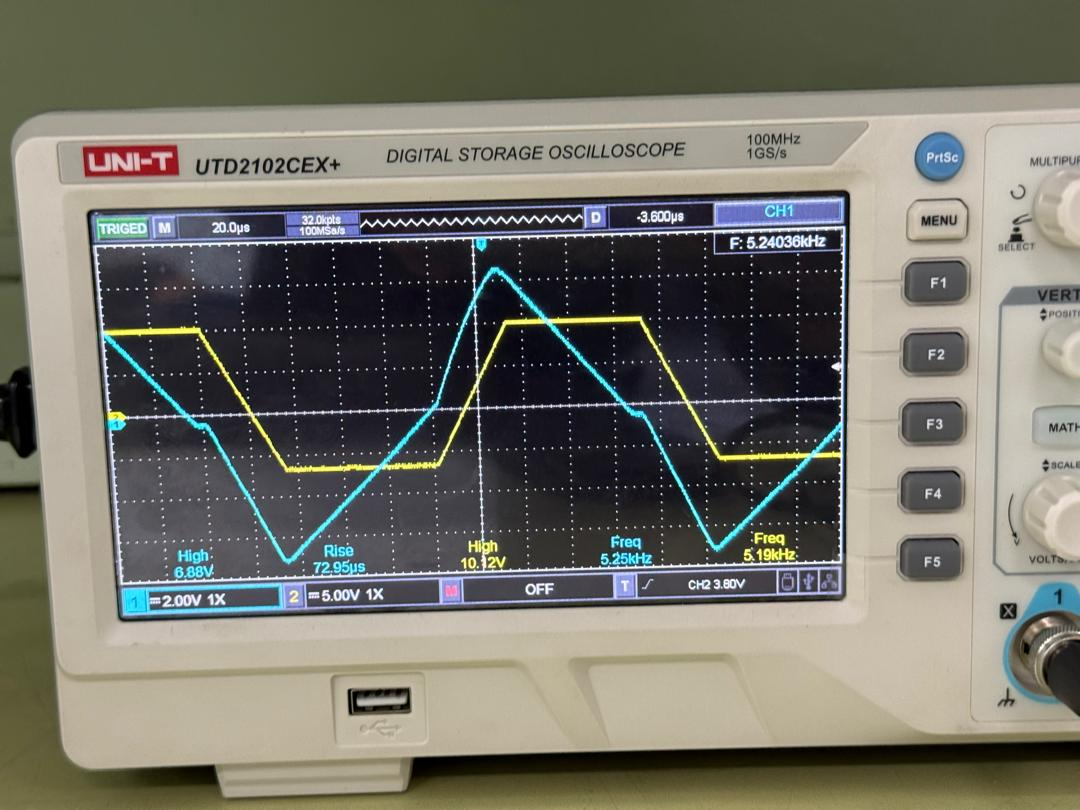
\includegraphics[width=0.6\textwidth]{resultados/generador-funciones-Vp.jpg}
    \caption{Medición de $V_p$ en el generador de funciones.}
    \label{ilus:generador-funciones-Vp}
\end{ilustracion}
